\documentclass[12pt, a4paper]{article}

\usepackage{import}
\usepackage{standalone}

\usepackage[top=4cm, right=2cm, bottom=2.7cm, left=2cm]{geometry}

\usepackage{wrapfig}
\usepackage{tabulary}
\usepackage{float}
\usepackage{pifont}
\usepackage{background}
\usepackage{tikz}


\pagestyle{empty}
\setlength{\parindent}{0pt}

\begin{document}
	\begin{minipage}{\textwidth}
		\section{Bloemen Planten \hfill\small Bron: Bebras}
			\begin{wrapfigure}{r}{0.3\textwidth} 
				
\includegraphics[width=\linewidth]{image1}
			\end{wrapfigure}
			Kleine bever en Grote bever planten bloemen in hun tuin. Kleine bever stapt met kleinere passen dan Grote bever en plant de bloemen ook dichter bij elkaar.
			
			In het begin staan de bevers rug aan rug en kijken in tegenovergestelde richting. Daarna stappen ze beide vooruit en volgen daarbij deze instructies:
			
\begin{lstlisting}[frame=single]
Herhaal twee keer:
	Plant een bloem aan je rechterkant
	Doe een stap vooruit
	Plant een bloem aan je linkerkant
	Doe een stap vooruit
\end{lstlisting}

			Hoe ziet de tuin eruit als de bevers klaar zijn?
		
			\begin{table}[H]
				\begin{tabulary}{\linewidth}{|C|C|C|C|}
					\hline
					\textbf{A} & \textbf{B} & \textbf{C} & \textbf{D} \\
					
\includegraphics[width=\linewidth]{option1} &
					
\includegraphics[width=\linewidth]{option2} &
					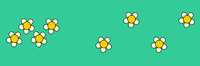
\includegraphics[width=\linewidth]{option3} &
					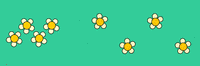
\includegraphics[width=\linewidth]{option4} \\
					\hline 
				\end{tabulary}
			\end{table}
	\end{minipage} \\ \\
		
\end{document}